\problemname{Cirkelskivevärlden}
Det är morgon på Cirkelskivevärlden, och solen håller på att gå upp.
Soluppgången på Cirkelskivevärlden är inte som soluppgångar på de flesta världar.
Detta är kanske inte så konstigt, då Cirkelskivevärlden inte är som de flesta världar (den är nämligen en cirkelskiva, till skillnad från de mer konventionella sfäriska världarna).
Cirkelskivevärlden är nämligen fylld med magi, och som alla vet undviker gärna solljuset att färdas genom starka magiska fält.

Som en av Cirkelskivevärldens mest kraftfulla magiker som bor på motsatt sida av Cirkelskivevärlden än där soluppgången först träffar cirkelskiveytan är detta ett faktum som du tycker är ytterst trevligt.
Du älskar nämligen sovmorgonar, och om du fick välja skulle solen helst stanna på sin sida av världen \emph{någon} timme längre på morgonarna.
Speciellt nu när du precis köpt ytterst solljuskänsliga hyacinther.
Turen i oturen ligger dock i att du som magiker kan påverka solljusets framfart över Cirkelskivevärlden genom att förstärka vissa av de magiska fält som finns i världen.

Världen kan modelleras som ett $n \times n$ rutnät, där alla rutor som ingår i en cirkelskiva kring rutnätets mitt existerar på världen (exakt vilka rutor som existerar ges av indata). 
I rutan på koordinat $(r, c)$ finns ett magiskt fält med styrkan $m_{r, c}$.
För att öka fältstyrkan med $1$ behöver du använda dig av $p_{r, c}$ trollformler på rutan.
Du kan inte öka fältstyrkan med mindre än $1$, men du kan öka den med $1$ upprepade gånger.

När solen går upp börjar den att försöka lysa upp position $(0, \frac{n - 1}{2})$ -- högst upp i rutnätet -- och sprider sig sedan på följande vis (se även figuren nedan).
Antag att solen försöker lysa upp en viss ruta $(r, c)$.
Det tar då $m_{r, c}$ sekunder innan solen lyser på rutan.
Så fort solen lyser på rutan börjar den försöka lysa på de (upp till fyra) rutor som rutan delar en kant med.

Du bor på rutan $(n-1, \frac{n-1}{2})$ (längst ner i rutnätet).
Totalt kan du $k$ stycken trollformler, som du vill använda dig av för att öka fältstyrkan på olika rutor i världen.
Din uppgift är att använda trollformlerna på ett sätt som maximerar antalet sekunder innan solen lyser upp rutan du bor på.

\section*{Indata}
\textbf{Observera:} testdatan på detta problem är \emph{öppen}. Du kan ladda ner den i menyn till höger (\texttt{1.in, 2.in, 3.in, 4.in, 5.in}).

Den första raden innehåller ett heltal $0 \le t \le 5$, ordningstalet för detta testfall.
Fallet $t = 0$ representar exempelfallet, och ska ignoreras (du kan skriva ut vad du vill då).

Den andra raden innehåller två heltal $n$ och $k$, där $n$ är udda.

De följande $n$ raderna innehåller talen $m_{r, c}$.
Den $i$:te raden innehåller talen $m_{i, c}$ för alla $0 \le c < n$.

De följande $n$ raderna innehåller talen $p_{r, c}$.
Den $i$:te raden innehåller talen $p_{i, c}$ för alla $0 \le c < n$.

Om en ruta inte är med på cirkelskivan är både $m_{r, c}$ och $p_{r, c}$ lika med $-1$, annars är de alltid positiva.

\section*{Utdata}
Skriv ut $n$ rader med $n$ tal vardera.
Den $i$:te raden ska innehålla antalet trollformler du använder på rutorna $(i, c)$ för $0 \le c < n$.
Antalet trollformler du använder på ruta $(i, c)$ måste vara en multipel av $p_{i, c}$.

\section*{Poängsättning}
Din lösning kommer att få poäng på varje av de fem testfallen.

Varje testfall poängsätts på följande vis.
Antag att tiden det tar för solen att nå dig är $T$ sekunder om inga trollformler används, att den maximala tiden någon deltagare lyckas åstadkomma är $T_{max}$ och att din tid är $T_{du}$.

Din poäng på testfallet är då

\[ 20 \cdot \frac{T_{du} - T}{T_{max} - T}. \]

Under tävlingen kommer $T_{max}$ vara satt till $2 \cdot T$.

\section*{Förklaring till exemplet}
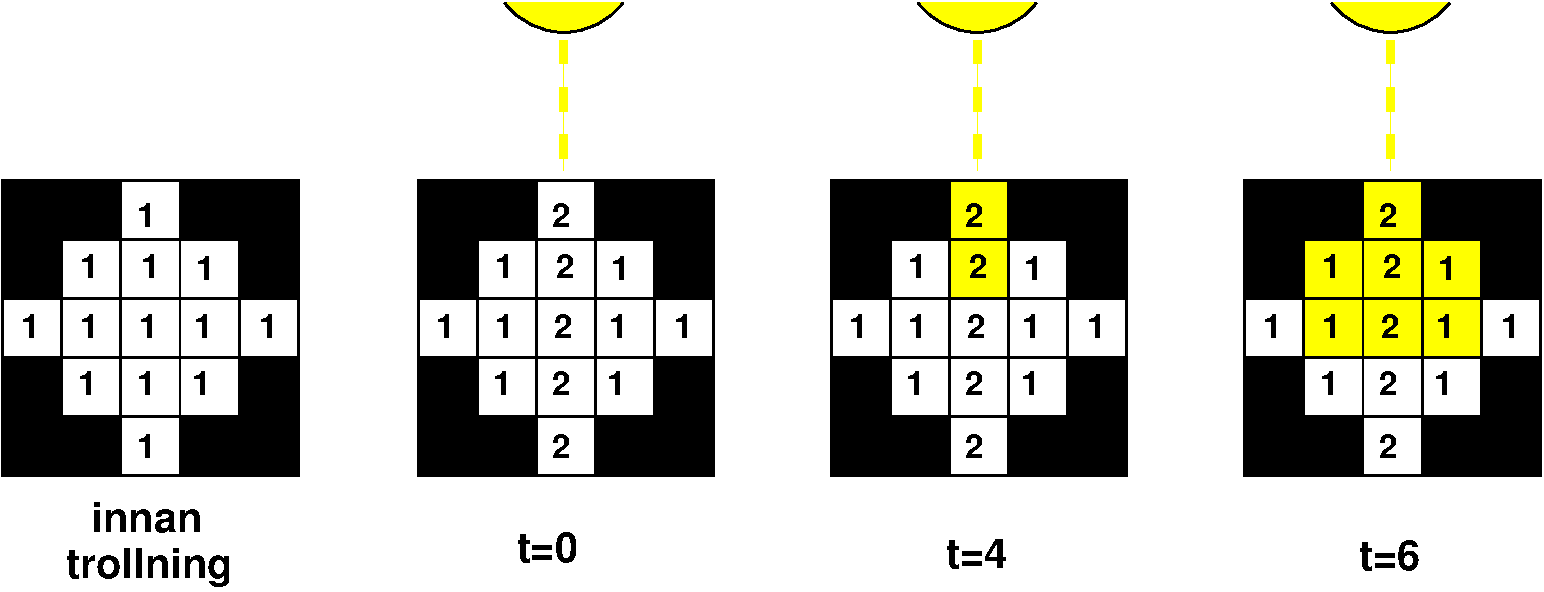
\includegraphics[width=14cm]{disc.pdf}\\
{\em Siffrorna anger den magiska fältstyrkan före trollningen (vänstra figuren) och efter trollningen (övriga figurer). Färgmarkeringen visar vilka rutor som är upplysta efter 0, 4 respektive 6 sekunder. Den nedersta rutan, där du bor, blir upplyst efter 10 sekunder. Det finns många andra sätt att trolla som ger samma fördröjning.}

